\section{统一共享内存}
接下来的两章将更深入地探讨如何管理数据。 有两种不同的方法可以相互补充:统一共享内存 (USM) 和Buffer。 
USM 公开了与Buffer不同的内存抽象级别 - USM 使用指针,而Buffer是更高级别的接口。 
本章重点介绍 USM。 下一章将重点讨论Buffer。

除非我们明确知道要使用Buffer,否则 USM 是一个不错的起点。 
USM 是一种基于指针的模型,允许通过常规 C++ 指针读写内存。

\subsection{为什么要使用USM?}
由于 USM 基于 C++ 指针,因此它是现有基于指针的 C++ 代码的自然起点。 
将指针作为参数的现有函数无需修改即可继续工作。 
在大多数情况下,唯一需要的更改是将现有的对 malloc 或 new 的调用替换为 USM 特定的分配例程,我们将在本章稍后讨论。

\subsection{分配类型}
虽然 USM 基于 C++ 指针,但并非所有指针都是一样的。 USM 定义了三种不同类型的分配,每种类型都有独特的语义。

设备可能不支持所有类型(甚至任何类型)的 USM 分配。

稍后我们将学习如何查询设备支持的内容。 图 6-1 总结了这三种类型的分配及其特点。

\begin{figure}[H]
	\centering
	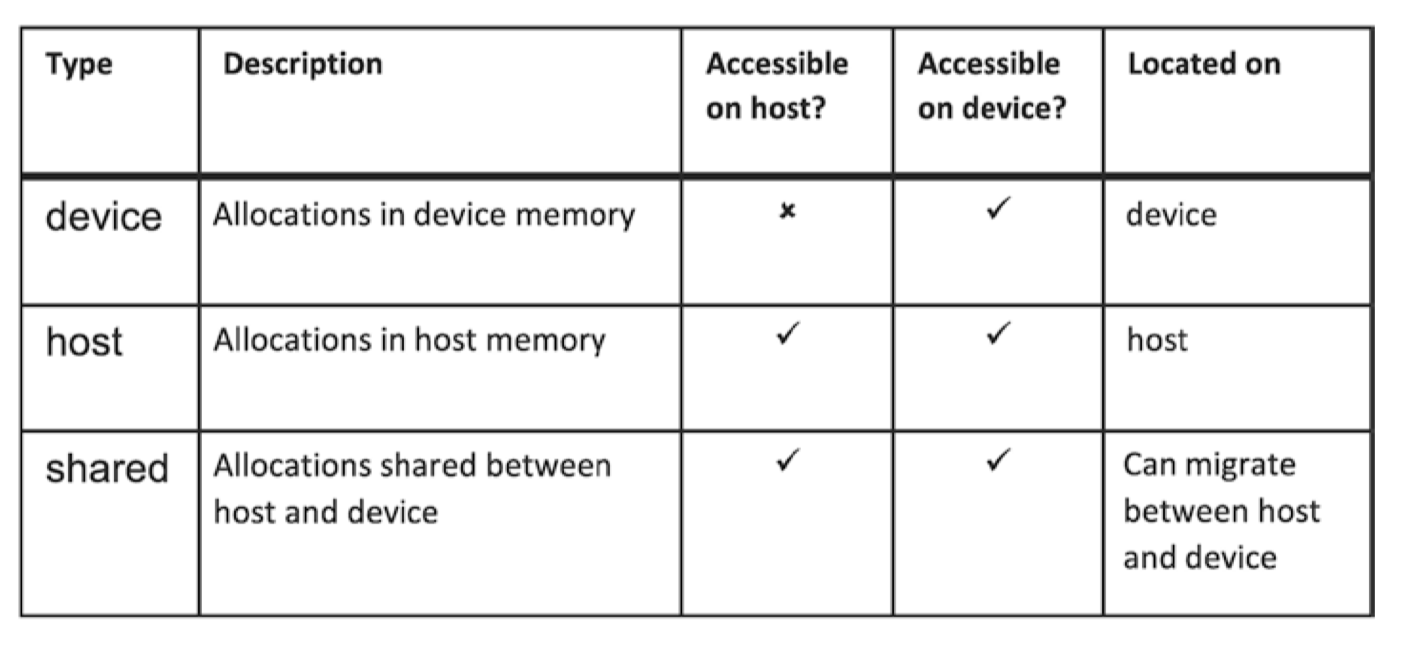
\includegraphics[width=0.9\textwidth]{figs/F6.1.png}
	\caption{\textit{USM 分配类型}}
\end{figure}

\subsubsection{设备分配}
为了获得指向设备附加内存(例如 (G)DDR 或 HBM)的指针,我们需要第一种类型的分配。 
设备分配可以由在特定设备上运行的Kernel读取或写入,但不能从主机上执行的代码直接访问它们(通常也不能由设备访问)。 
尝试访问主机上的设备分配可能会导致数据不正确或程序因错误而崩溃。 
我们必须使用显式 USM memcpy 机制在主机和设备之间复制数据,
该机制指定必须在两个位置之间复制多少数据,这将在本章后面介绍。

\subsubsection{主机分配}
第二种类型的分配比设备分配更容易使用,因为我们不必在主机和设备之间手动复制数据。 
主机分配是主机内存中的分配,主机和设备均可访问。 这些分配虽然可以在设备上访问,但无法迁移到设备的附加内存。 
相反,Kernel可以远程读取或写入该内存,通常通过 PCI Express 等较慢的总线(或者如果它是 CPU 设备或集成 GPU 设备,
则实际上没有什么不同)。 这种便利性和性能之间的权衡是我们必须考虑的。 
尽管主机分配可能会产生更高的访问成本,但仍然有充分的理由使用它们。 
示例包括很少访问的数据、无法放入设备附加内存的大型数据集,或者设备可能不支持共享分配等替代方案(如下所述)。

\subsubsection{共享分配}
最终类型的分配结合了设备和主机分配的属性,将主机分配的程序员便利性与设备分配提供的更高性能结合起来。 
与主机分配一样,共享分配可以在主机和设备上访问。 
它们之间的区别在于,共享分配可以自动在主机内存和设备附加内存之间自由迁移,无需我们干预。 
如果分配已迁移到设备,则在该设备上执行的任何访问该设备的Kernel都会比从主机远程访问该设备具有更高的性能。 
然而,共享分配并不能给我们带来所有好处而没有任何缺点。

自动迁移可以通过多种方式实现。 无论运行时选择哪种方式实现共享分配,它们通常都会付出延迟增加的代价。 
通过设备分配,我们可以准确地知道需要复制多少内存,并可以安排复制尽早开始。 
自动迁移机制无法预见未来,并且在某些情况下,在Kernel尝试访问数据之前不会开始移动数据。 
然后,Kernel必须等待或阻塞,直到数据移动完成才能继续执行。 
在其他情况下,运行时可能无法确切知道Kernel将访问多少数据,
并且可能会保守地移动比所需数量更大的数据,这也会增加Kernel的延迟。

我们还应该注意,虽然共享分配可以迁移,但这并不一定意味着 SYCL 的所有实现都会迁移它们。 
我们期望大多数实现通过迁移来实现共享分配,但某些设备可能更愿意以与主机分配相同的方式实现它们。 
在这样的实现中,分配在主机和设备上仍然可见,但我们可能看不到迁移实现可以提供的性能增益。

\subsection{分配内存}
USM 允许我们以各种不同的方式分配内存,以满足不同的需求和偏好。 
然而,在我们更详细地讨论所有方法之前,我们应该讨论 USM 分配与常规 C++ 分配有何不同。

\subsubsection{我们需要知道什么?}
常规 C++ 程序可以通过多种方式分配内存:new、malloc 或分配器。 
无论我们喜欢哪种语法,内存分配最终都是由主机操作系统中的系统分配器执行的。 
当我们在 C++ 中分配内存时,唯一关心的是“我们需要多少内存?” 和“有多少内存可供分配?” 
然而,USM 在执行分配之前需要额外的信息。

首先,USM 分配需要指定所需的分配类型:设备、主机或共享。 为了获得所需的行为,请求正确的分配类型非常重要。 
接下来,每个 USM 分配都必须指定一个将针对其进行分配的上下文对象。 书中的大多数示例都传递队列对象(然后提供上下文)。 
到目前为止,上下文对象在本书中还没有进行太多讨论,因此值得在这里稍微讨论一下。 
上下文代表我们可以在其上执行Kernel的一个设备或一组设备。 
我们可以将上下文视为运行时存储有关其正在执行的操作的某些状态的方便位置。 
除了在大多数 SYCL 程序中传递上下文之外,程序员不太可能直接与上下文交互。 
我们确实在第 13 章中提供了一些有关上下文的提示。

不保证 USM 分配可在不同上下文中使用 - 所有 USM 分配、队列和Kernel共享相同的上下文对象非常重要。 
通常,我们可以从用于向设备提交工作的队列中获取此上下文。

最后,设备分配(以及一些共享分配)还要求我们指定哪个设备将为分配提供内存。 
这很重要,因为我们不想超额订阅设备的内存(除非设备能够支持这一点——我们将在本章后面讨论数据迁移时详细介绍这一点)。 
USM 分配例程可以通过添加这些额外参数来区别于它们的 C++ 类似例程。

\subsubsection{多种风格}
有时,试图用单一选项取悦所有人被证明是一项不可能完成的任务,就像有些人喜欢咖啡而不是茶,或者 emacs 而不是 vi 一样。 
如果我们问程序员分配接口应该是什么样子,我们会得到几个不同的答案。 
USM 拥抱这种选择的多样性,并提供几种不同风格的分配接口。 
这些不同的风格是 C 风格、C++ 风格和 C++ 分配器风格。 我们现在将讨论每一个并指出它们的相似点和不同点。

\paragraph{按 C 进行分配}

\begin{figure}[H]
	\centering
	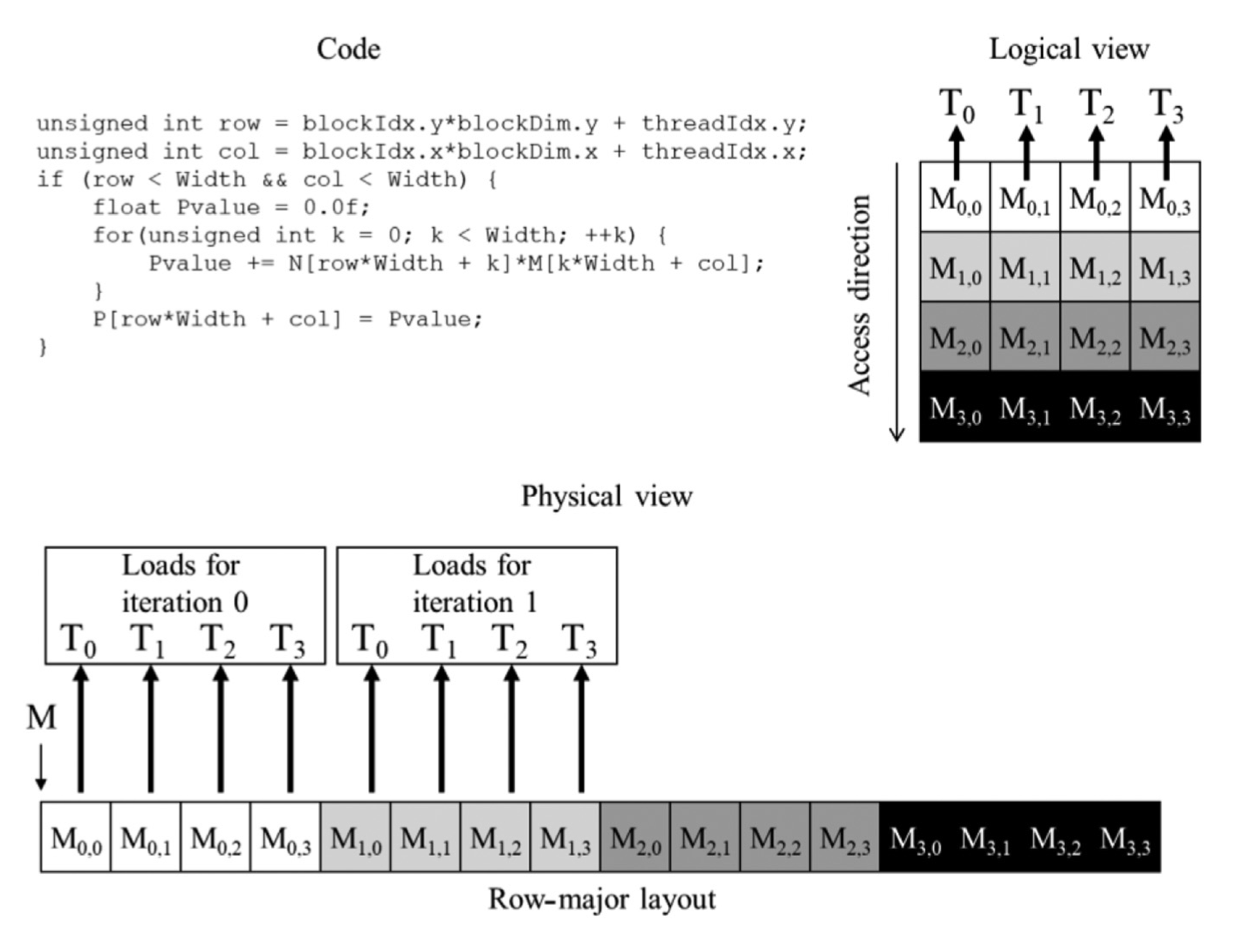
\includegraphics[width=0.9\textwidth]{figs/F6.2.png}
	\caption{\textit{C 风格的 USM 分配函数}}
\end{figure}

第一种类型的分配函数(在图 6-2 中列出,
稍后在图 6-6 和 6-7 所示的示例中使用)是根据 C 中的内存分配进行建模的:malloc 函数需要多个字节来分配
并返回一个 void*指针。 这种风格的函数与类型无关。 我们必须指定要分配的总字节数,
这意味着如果我们想要分配 N 个 X 类型的对象,则必须要求 N * sizeof(X) 总字节数。 
返回的指针是 void * 类型,这意味着我们必须将其转换为指向 X 类型的适当指针。
这种样式非常简单,但由于所需的大小计算和类型转换,可能会很冗长。

我们可以将这种分配方式进一步分为两类:命名函数和单一函数。 这两种风格之间的区别在于我们如何指定所需的 USM 分配类型。 
对于命名函数(malloc\_device、malloc\_host 和 malloc\_shared),USM 分配的类型在函数名称中进行编码。 
单一函数 malloc 需要将 USM 分配的类型指定为附加参数。 两种口味并不比另一种更好,选择哪种口味取决于我们的喜好。

如果不简要提及对齐,我们就无法继续前进。 每个版本的 malloc 也有一个aligned\_alloc 对应项。 
malloc 函数返回与我们设备的默认行为一致的内存。 
成功时,它将返回一个具有有效对齐方式的合法指针,但在某些情况下,我们可能更愿意手动指定对齐方式。 
在这些情况下,我们应该使用aligned\_alloc变体之一,它也要求我们指定所需的分配对齐方式。 
标准对齐是2的幂次。 值得注意的是,在许多设备上,分配最大程度地对齐以对应于硬件的功能,
因此,虽然我们可能要求分配为 4、8、16 或 32 字节对齐,但实际上我们可能会看到更大的分配空间。 
对齐可以满足我们的要求,然后是一些。

\paragraph{C++ 的分配}

\begin{figure}[H]
	\centering
	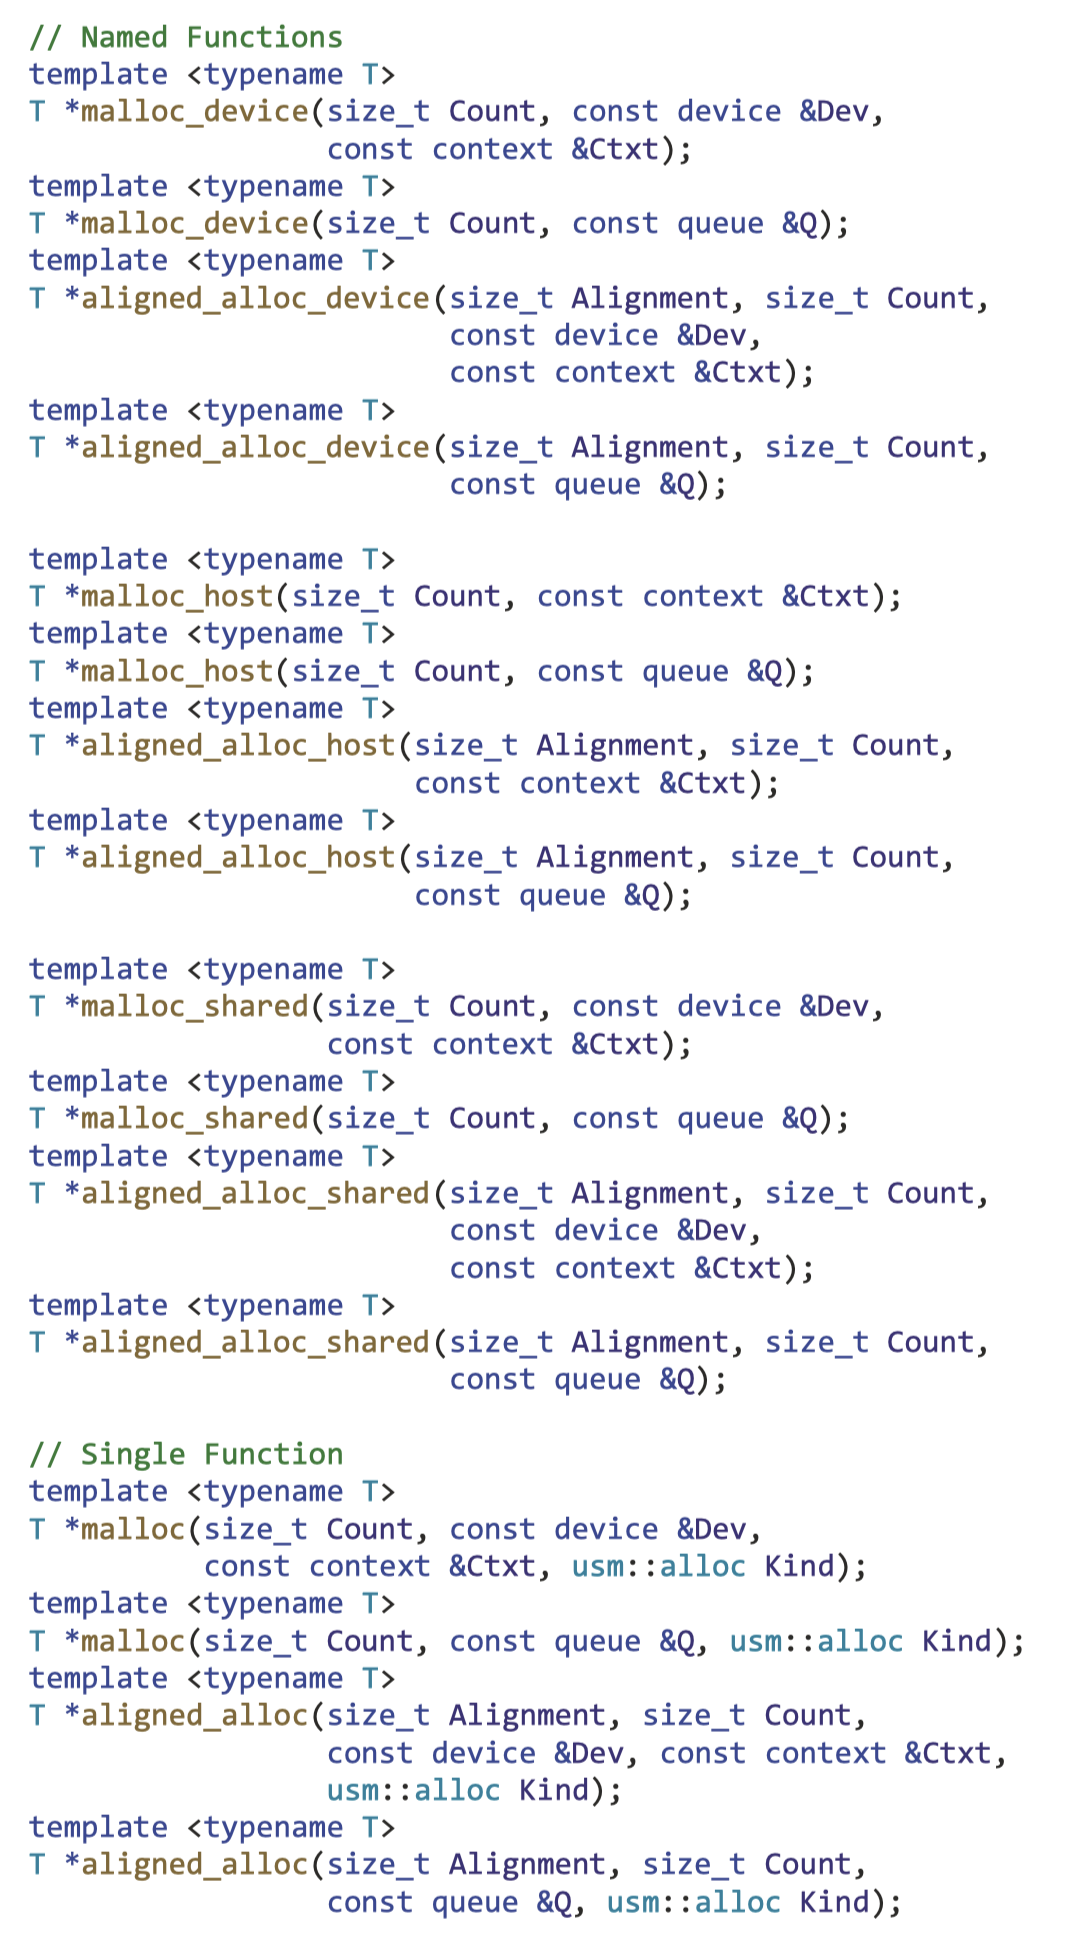
\includegraphics[width=0.9\textwidth]{figs/F6.3.png}
	\caption{\textit{C++ 风格的 USM 分配函数}}
\end{figure}

USM 分配函数的下一个风格(图 6-3 中列出)与第一个风格非常相似,但更多的是 C++ 外观和感觉。 
我们再次拥有分配例程的命名版本和单函数版本,以及默认的和用户指定的对齐版本。 
不同之处在于,现在我们的函数是 C++ 模板函数,它分配 T 类型的 Count 对象并返回 T * 类型的指针。 
利用现代 C++ 可以简化事情,因为我们不再需要手动计算分配的总大小(以字节为单位)或将返回的指针转换为适当的类型。 
这也往往会在代码中产生更紧凑且不易出错的表达式。 
然而,我们应该注意到,与 C++ 中的“new”不同,
malloc 风格的接口不会为正在分配的对象调用构造函数——我们只是分配足够的字节来适合该类型。

对于考虑到 USM 编写的新代码来说,这种分配方式是一个很好的起点。 
对于已经大量使用 C 或 C++ malloc 的现有 C++ 代码,前面的 C 风格是一个很好的起点,我们将在其中添加 USM 的使用。

\paragraph{C++ 分配器}

\begin{figure}[H]
	\centering
	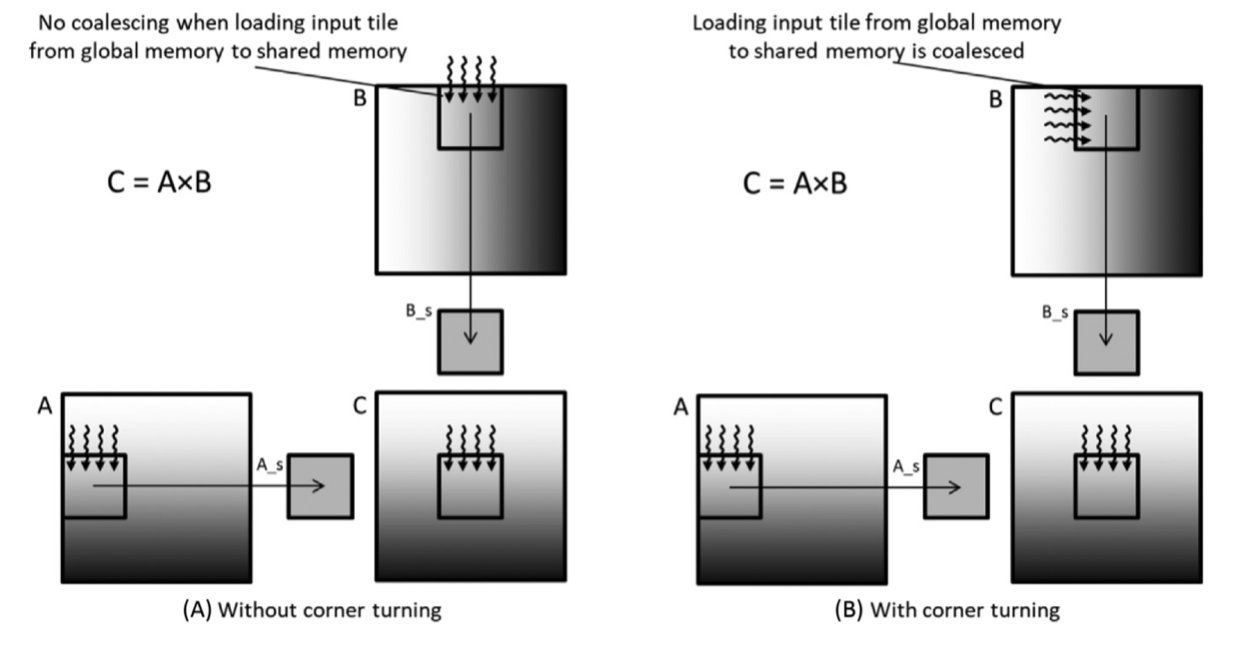
\includegraphics[width=0.9\textwidth]{figs/F6.4.png}
	\caption{\textit{C++ 分配器风格的 USM 分配函数}}
\end{figure}

USM 分配的最终风格(图 6-4)甚至比以前的风格更多地拥抱现代 C++。 
这种风格基于 C++ 分配器接口,它定义了用于在容器(例如 std::vector)内直接或间接执行内存分配的对象。 
如果我们的代码大量使用容器对象,可以向用户隐藏内存分配和释放的详细信息,
从而简化代码并减少出现错误的机会,则这种分配器风格非常有用。

\subsubsection{释放内存}
无论程序分配什么,最终都必须被释放。 
USM 定义了一种 free 方法来释放由 malloc 或aligned\_malloc 函数之一分配的内存。 
此 free 方法还将分配内存的上下文作为额外参数。 队列也可以代替上下文。 
如果内存是使用 C++ 分配器对象分配的,则也应该使用该对象来释放内存。

\subsubsection{分配示例}

\begin{figure}[H]
	\centering
	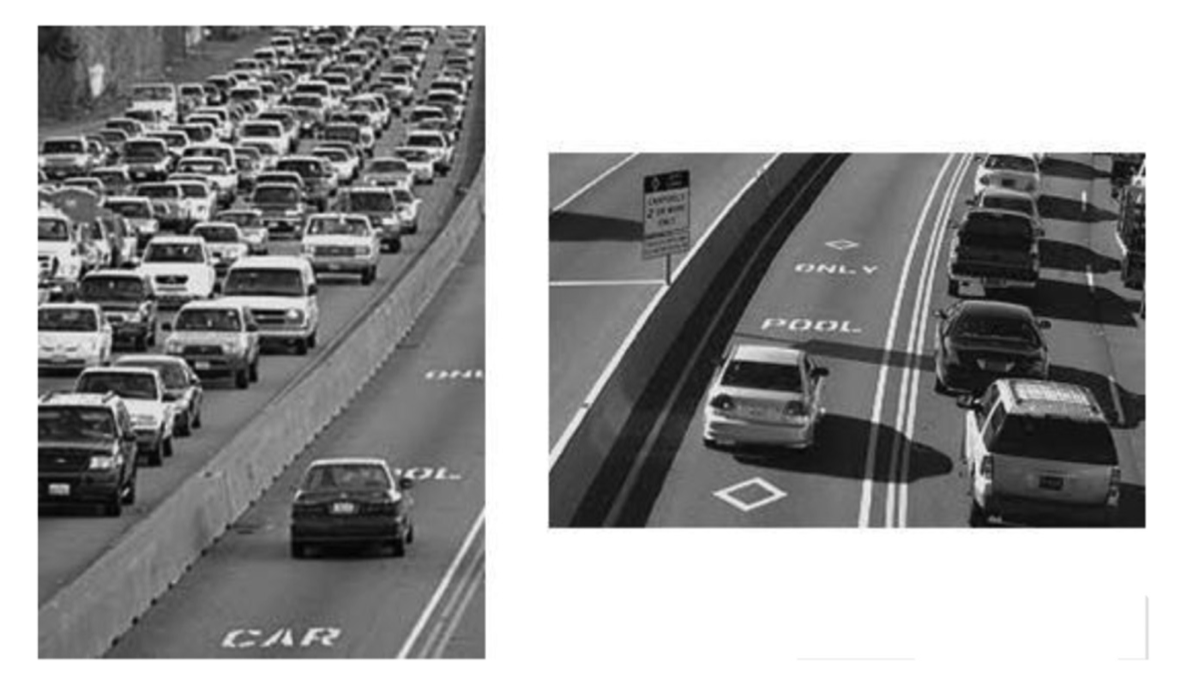
\includegraphics[width=0.9\textwidth]{figs/F6.5.png}
	\caption{\textit{三种风格的分配方式}}
\end{figure}

在图 6-5 中,我们展示了如何使用刚才描述的三种样式执行相同的分配。 
在此示例中,我们将 N 个单精度浮点数分配为共享分配。 第一个分配 f1 使用 C 风格的 void * 返回 malloc 例程。 
对于此分配,我们显式传递从队列中获取的设备和上下文。 我们还必须将结果转换回 float *。 
第二个分配 f2 执行相同的操作,但使用 C++ 样式模板化 malloc。 
由于我们将元素的类型 float 传递给分配例程,因此我们只需要指定要分配的浮点数量,并且不需要转换结果。 
我们还使用采用队列而不是设备和上下文的形式,产生一个非常简单和紧凑的语句。 
第三个分配 f3 使用 USM C++ 分配器类。 我们实例化适当类型的分配器对象,然后使用该对象执行分配。 
最后,我们展示如何正确地释放每个分配。

\subsection{数据管理}
现在我们了解了如何使用 USM 分配内存,我们将讨论如何管理数据。 
我们可以将其分为两部分:数据初始化和数据移动。

\subsubsection{初始化}
数据初始化涉及在执行计算之前用值填充我们的内存。 常见初始化模式的一个示例是在使用分配之前用零填充分配。 
如果我们要使用 USM 分配来做到这一点,我们可以通过多种方式来做到这一点。 
首先,我们可以编写一个Kernel来执行此操作。 如果我们的数据集特别大或者初始化需要复杂的计算,
这是一种合理的方法,因为初始化可以并行执行(并且它使初始化的数据准备好在设备上运行)。 
其次,我们可以将其实现为主机代码中对分配的所有元素进行循环,将每个元素设置为零。 
然而,这种方法可能存在一个问题。 循环对于主机和共享分配来说效果很好,因为这些可以在主机上访问。 
但是,由于主机上无法访问设备分配,因此主机代码中的循环将无法写入它们。 这给我们带来了第三种选择。

memset 函数旨在有效地实现此初始化模式。 USM 提供了 memset 的一个版本,它是处理程序类和队列类的成员函数。 
它需要三个参数:表示我们要设置的内存基地址的指针、表示要设置的字节模式的字节值以及要设置到该模式的字节数。 
与主机上的循环不同,memset 并行发生,并且也适用于设备分配。

虽然 memset 是一个有用的操作,但它只允许我们指定一个字节模式来填充分配,这一事实是相当有限的。 
USM 还提供了一个 fill 方法(作为处理程序和队列类的成员),让我们可以用任意模式填充内存。 
fill 方法是一个以我们要写入分配的模式类型为模板的函数。 
使用 int 对其进行模板化,我们可以用 32 位整数“42”填充分配。 
与 memset 类似,fill 接受三个参数:指向要填充的分配基地址的指针、要填充的值以及我们想要将该值写入分配的次数。

\subsubsection{数据移动}
数据移动可能是 USM 需要理解的最重要的方面。 
如果正确的数据没有在正确的时间出现在正确的位置,我们的程序将产生错误的结果。 
USM 定义了两种可用于管理数据的策略:显式策略和隐式策略。 
我们想要使用哪种策略的选择与我们的硬件支持或我们想要使用的 USM 分配类型有关。

\paragraph{显式的}

\begin{figure}[H]
	\centering
	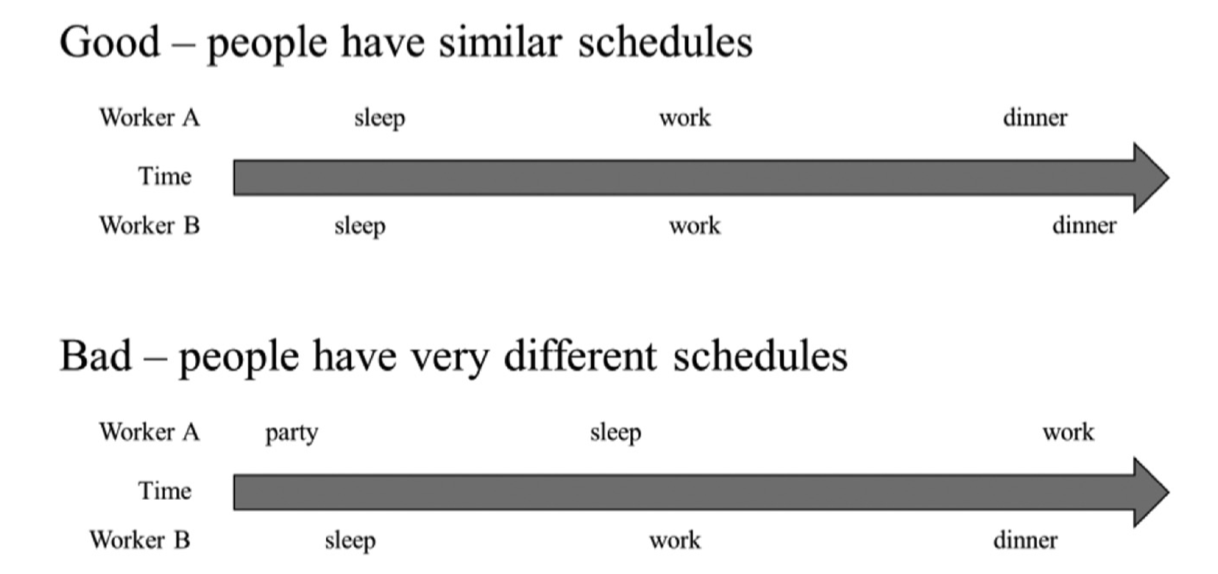
\includegraphics[width=0.9\textwidth]{figs/F6.6.png}
	\caption{\textit{USM 显式数据移动示例}}
\end{figure}

USM 提供的第一个策略是显式数据移动(图 6-6)。

在这里,我们必须在主机和设备之间显式复制数据。 我们可以通过调用处理程序类和队列类上的 memcpy 方法来做到这一点。 
memcpy 方法采用三个参数:指向目标内存的指针、指向源内存的指针以及要在主机和设备之间复制的字节数。 
我们不需要指定复制发生的方向——这隐含在源指针和目标指针中。

显式数据移动的最常见用法是在 USM 中的设备分配之间进行复制,因为它们在主机上无法访问。 
必须插入显式数据复制确实需要我们付出努力。 
此外,它可能是错误的来源:副本可能会被意外省略、复制的数据量可能不正确、或者源或目标指针可能不正确。

然而,显式数据移动不仅有缺点。 它给我们带来了巨大的优势:完全控制数据移动。 
控制复制数据量和复制数据的时间对于在某些应用程序中实现最佳性能非常重要。 
理想情况下,我们可以尽可能将计算与数据移动重叠,确保硬件以高利用率运行。

其他类型的 USM 分配(主机分配和共享分配)都可以在主机和设备上访问,并且不需要显式复制到设备。 
这引出了 USM 中数据移动的另一种策略。

\paragraph{隐式的}

\begin{figure}[H]
	\centering
	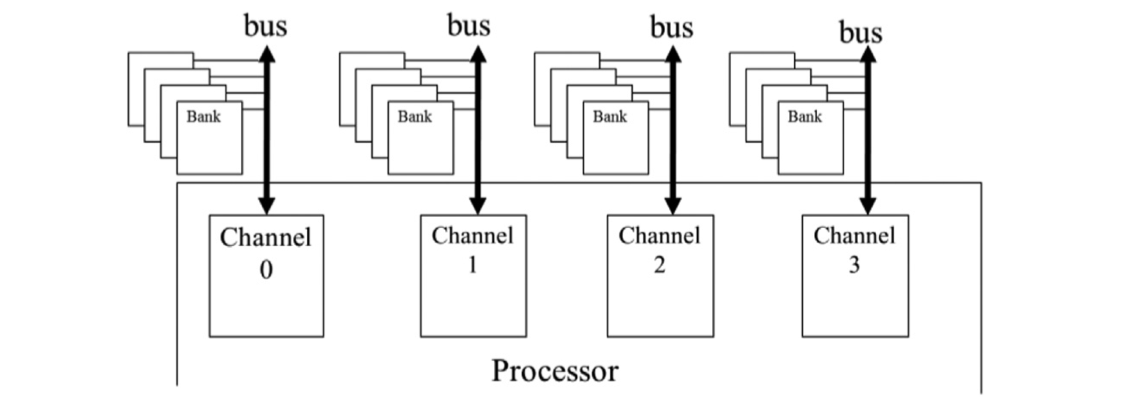
\includegraphics[width=0.9\textwidth]{figs/F6.7.png}
	\caption{\textit{USM 隐式数据移动示例}}
\end{figure}

USM 提供的第二种策略是隐式数据移动(示例用法如图 6-7 所示)。 
在这种策略中,数据移动是隐式发生的,也就是说,不需要我们的输入。 
通过隐式数据移动,我们不需要插入对 memcpy 的调用,因为我们可以在任何想要使用数据的地方通过 USM 指针直接访问数据。 
相反,系统的工作是确保数据在使用时在正确的位置可用。

对于主机分配,人们可能会争论它们是否真的会导致数据移动。 
由于根据定义,它们始终保留指向主机内存的指针,因此给定主机指针表示的内存无法存储在设备上。 
但是,当在设备上访问主机分配时,确实会发生数据移动。 
我们读取或写入的值不是通过适当的接口传入或传出Kernel,而是将内存迁移到设备。 
这对于数据不需要保留在设备上的流Kernel非常有用。

隐式数据移动主要涉及 USM 共享分配。 这种类型的分配在主机和设备上都可以访问,更重要的是,可以在主机和设备之间迁移。 
关键点是,这种迁移只需访问不同位置的数据即可自动或隐式发生。 
接下来,我们将讨论共享分配的数据迁移时需要考虑的几个问题。

\paragraph{迁移}

通过显式数据移动,我们可以控制发生的数据移动量。 通过隐式数据移动,系统可以为我们处理这个问题,但可能效率不高。 
SYCL 运行时不是预言机,它无法在应用程序执行操作之前预测将访问哪些数据。 
此外,指针分析对于编译器来说仍然是一个非常困难的问题,编译器可能无法准确地分析和识别Kernel内部可能使用的每个分配。 
因此,隐式数据移动机制的实现可能会根据支持 USM 的设备的功能做出不同的决策,这会影响共享分配的使用方式及其执行方式。

如果设备功能非常强大,它可能能够按需迁移内存。 
在这种情况下,数据移动将在主机或设备尝试访问当前不在所需位置的分配之后发生。 
按需数据极大地简化了编程,因为它提供了所需的语义,即 USM 共享指针可以在任何地方访问并且正常工作。 
如果设备不支持按需迁移(第 12 章解释了如何查询设备的功能),
它可能仍然能够保证相同的语义,并对如何使用共享指针进行额外限制。

USM 共享分配的限制形式控制何时何地可以访问共享指针以及共享分配的大小。 
如果设备无法按需迁移内存,则意味着运行时必须保守,
并假设Kernel可以访问其设备附加内存中的任何分配。 这会带来一些后果。

首先,这意味着主机和设备不应尝试同时访问共享分配。 应用程序应该分阶段交替访问。 
主机可以访问分配,然后Kernel可以使用该数据进行计算,最后主机可以读取结果。 
如果没有此限制,主机可以自由访问分配的不同部分,而不是Kernel当前正在访问的部分。 
这种并发访问通常发生在设备内存页的粒度上。 主机可以访问一个页,而设备可以访问另一页。 
以原子方式访问同一条数据将在第 19 章中介绍。程序员可以查询设备是否受到此限制,稍后我们将详细了解设备查询机制。

这种限制形式的共享分配的下一个后果是分配受到连接到设备的内存总量的限制。 
如果设备无法按需迁移内存,则它无法将数据迁移到主机以腾出空间来引入不同的数据。 
如果设备确实支持按需迁移,则可以超额订阅其连接的内存,
从而允许Kernel计算比设备内存通常可以容纳的数据更多的数据,尽管这种灵活性可能会因额外的数据移动而带来性能损失。

\paragraph{细粒度控制}

当设备支持共享分配的按需迁移时,在当前未驻留的位置访问内存后,会发生数据移动。 
但是,Kernel在等待数据移动完成时可能会停止。 它执行的下一条语句甚至可能会导致发生更多数据移动,
并给Kernel执行带来额外的延迟。

\begin{figure}[H]
	\centering
	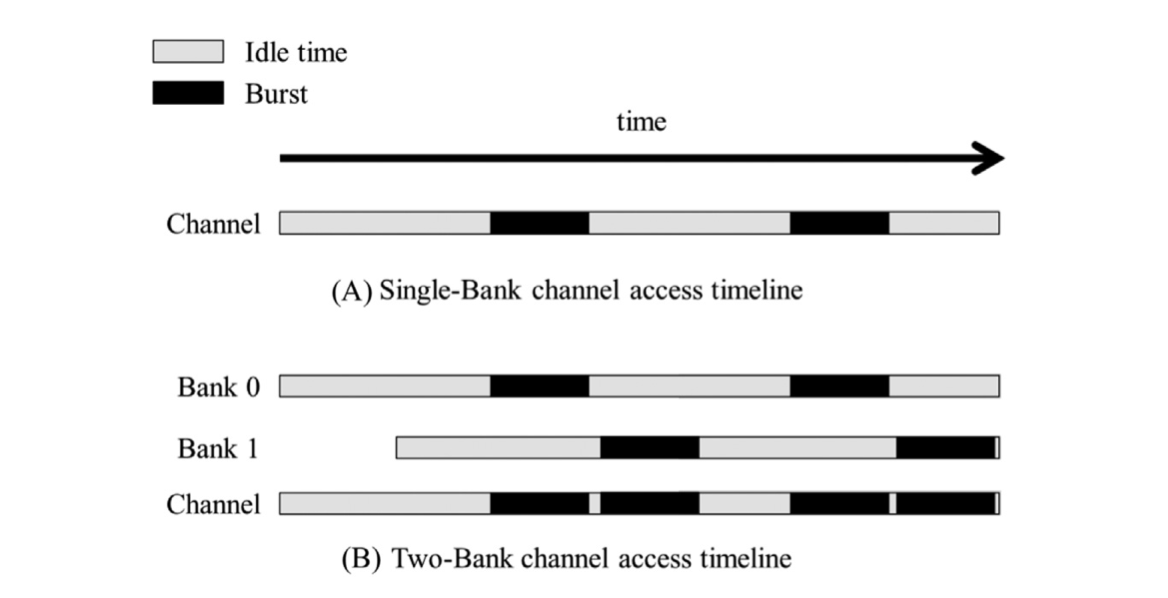
\includegraphics[width=0.9\textwidth]{figs/F6.8.png}
	\caption{\textit{通过 prefetch 和 mem\_advise 进行细粒度控制}}
\end{figure}

SYCL 为我们提供了一种修改自动迁移机制性能的方法。 它通过定义两个函数来实现这一点:prefetch 和 mem\_advise。 
图 6-8 显示了每种方法的简单用法。 这些函数让我们向运行时提供有关Kernel如何访问数据的提示,
以便运行时可以选择在Kernel尝试访问数据之前开始移动数据。 
请注意,此示例使用队列快捷方式方法,直接在队列对象上调用parallel\_for,
而不是在传递给submit 方法(命令组)的 lambda 内部调用。

我们做到这一点的最简单方法是调用预取。 该函数作为处理程序或队列类的成员函数进行调用,并采用基指针和字节数。 
这让我们可以通知运行时某些数据即将在设备上使用,以便它可以立即开始迁移它。 
理想情况下,我们会尽早发出这些预取提示,以便当Kernel接触数据时,它已经驻留在设备上,从而消除了我们之前描述的延迟。

SYCL 提供的另一个函数是 mem\_advise。 此函数允许我们提供有关如何在Kernel中使用内存的特定于设备的提示。 
我们可以指定的此类可能建议的一个示例是数据将仅在Kernel中读取,而不是写入。 
在这种情况下,系统可以意识到它可以复制设备上的数据,以便在Kernel完成后不需要更新主机的版本。 
但是,传递给 mem\_advise 的建议特定于特定设备,因此在使用此函数之前请务必检查硬件文档。

\subsection{查询}
最后,并非所有设备都支持 USM 的所有功能。 
如果我们希望我们的程序可以跨不同设备移植,我们不应该假设所有 USM 功能都可用。 
USM 定义了一些我们可以查询的内容。 这些查询可以分为两类:指针查询和设备能力查询。 
图 6-9 显示了每种方法的简单用法。

\begin{figure}[H]
	\centering
	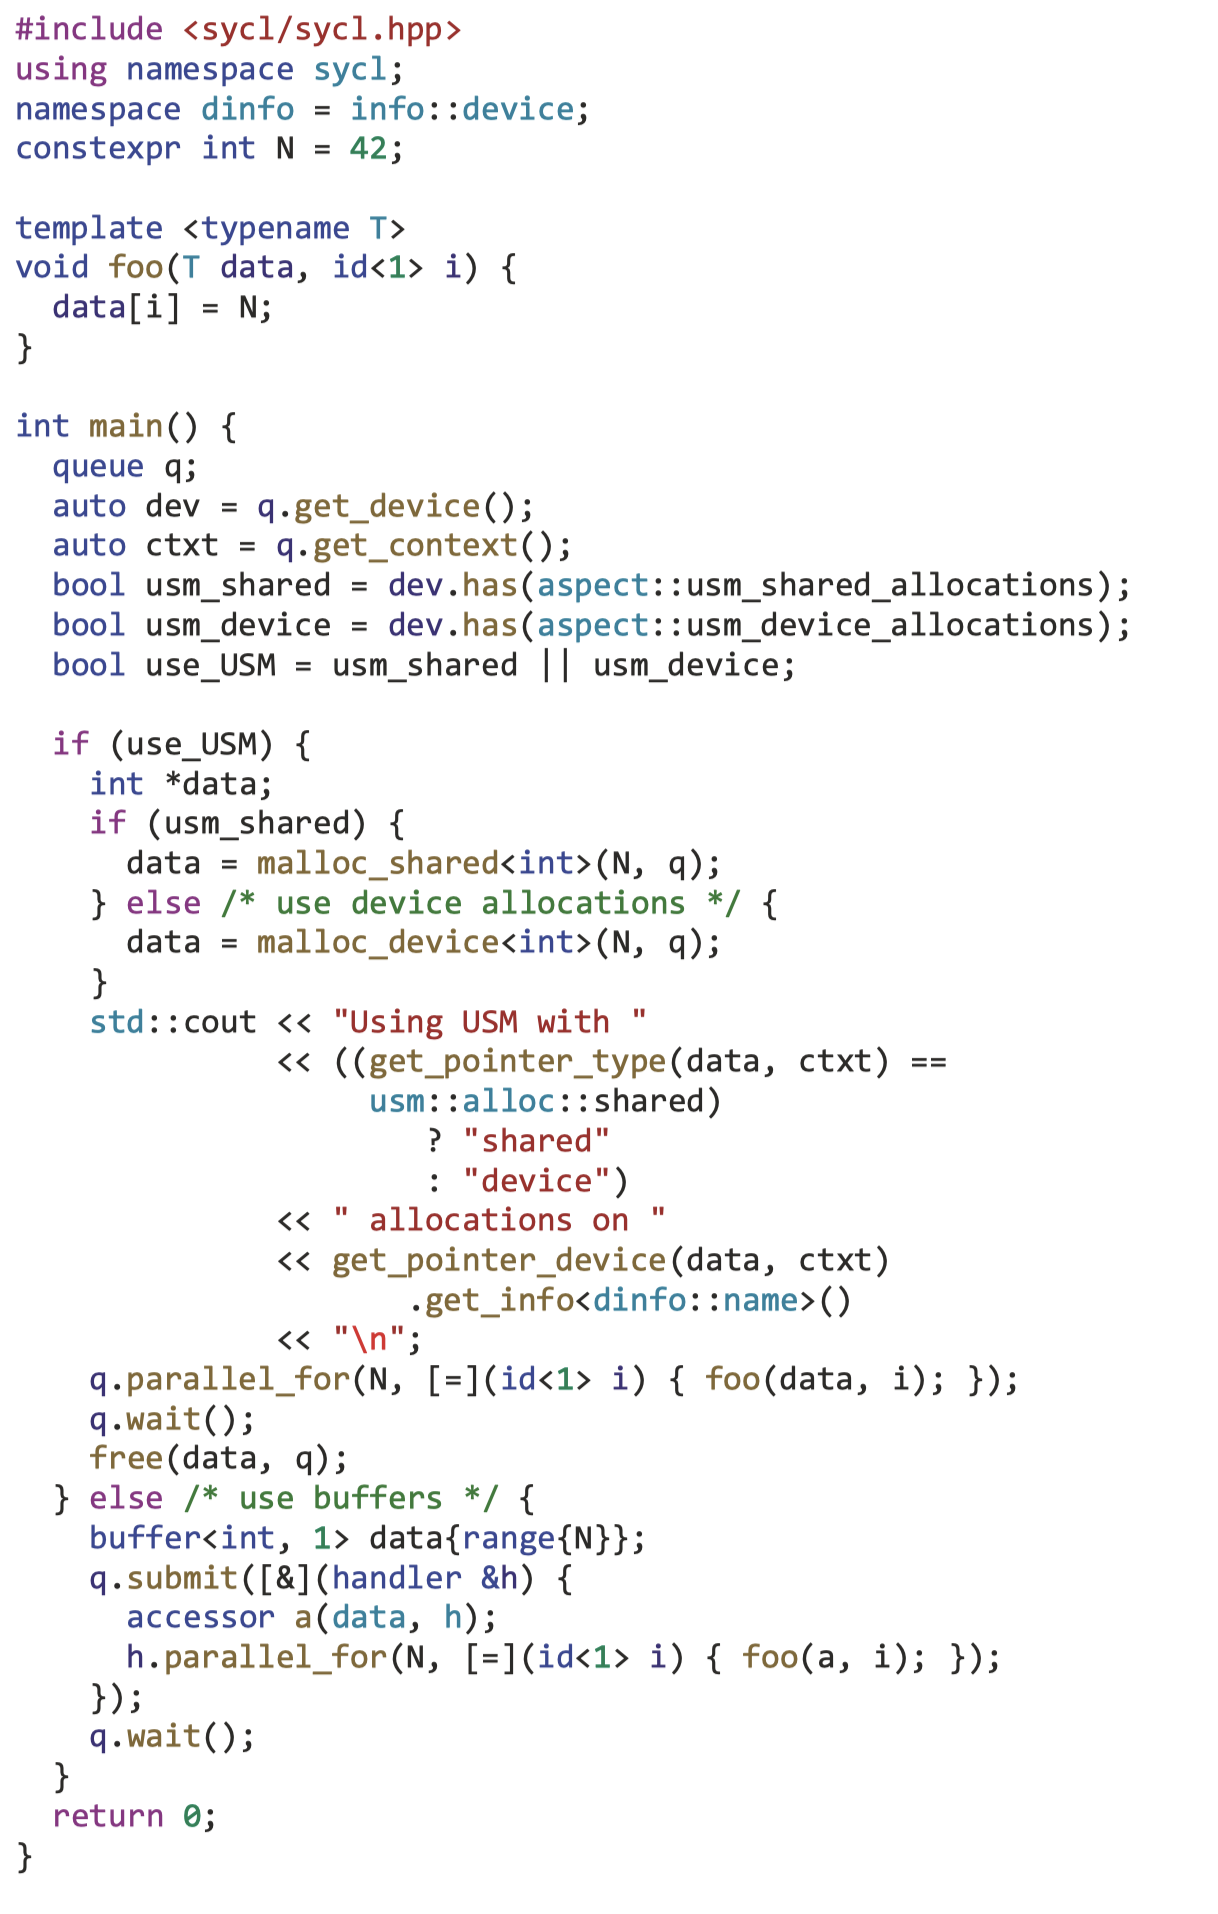
\includegraphics[width=0.9\textwidth]{figs/F6.9.png}
	\caption{\textit{对 USM 指针和设备的查询}}
\end{figure}

USM 中的指针查询回答两个问题。 
第一个问题是“这个指针指向什么类型的USM分配?” get\_pointer\_type 函数采用指针和 SYCL 上下文,
并返回 usm::alloc 类型的结果,该结果可以有四个可能的值:主机、设备、共享或未知。 
第二个问题是“这个 USM 指针分配给什么设备?” 我们可以将指针和上下文传递给函数 get\_pointer\_device 并获取设备对象。 
这主要用于设备或共享 USM 分配,因为它对于主机分配没有多大意义。 
SYCL 规范规定,当与主机分配一起使用时,将返回上下文中的第一个设备 - 除了避免引发异常之外,
这没有任何特殊原因,这对于可能在 USM 分配上模板化的代码来说似乎有点奇怪 类型。

USM 提供的第二种类型的查询涉及设备的功能。 USM 有自己的设备方面列表,可以通过调用设备对象上的 has 来查询。 
这些查询可用于测试设备支持哪些类型的 USM 分配。 此外,我们可以查询主机和设备是否可以同时访问共享分配。 
完整的查询列表如图 6-10 所示。 在第12章中,我们将更详细地了解查询机制。

\begin{figure}[H]
	\centering
	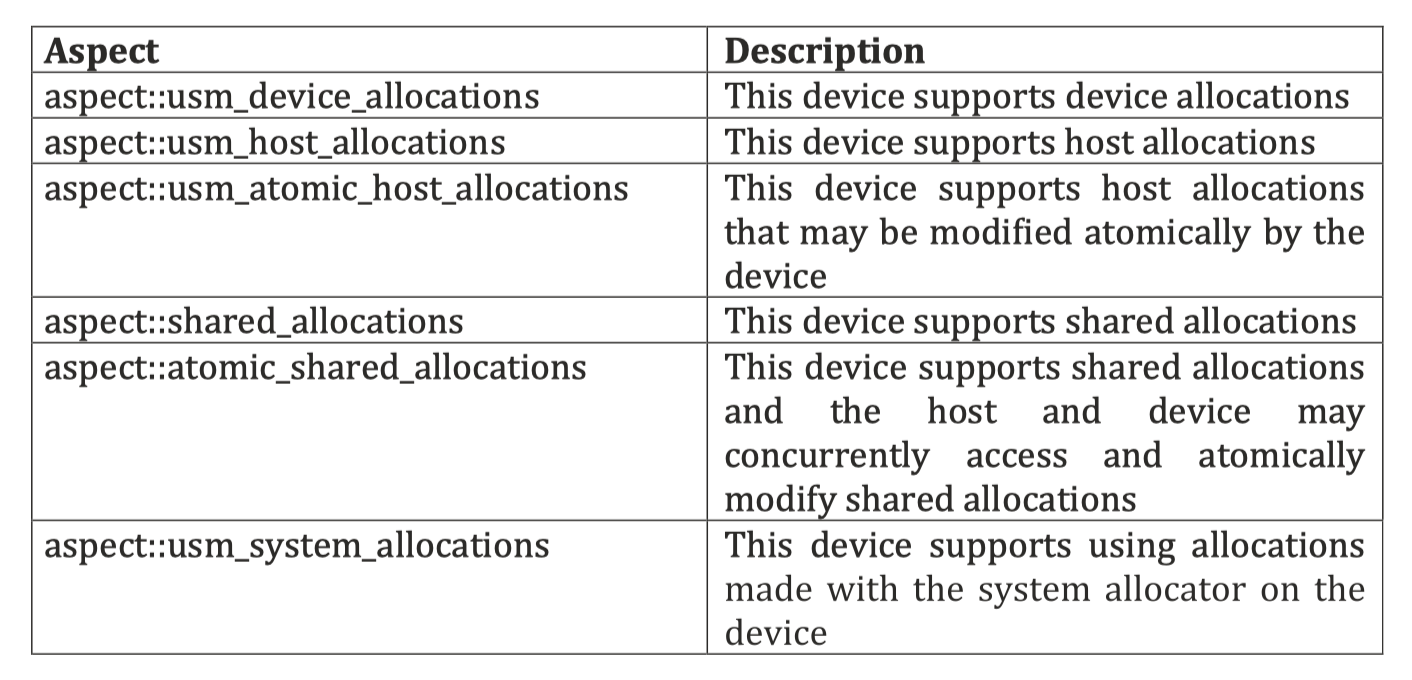
\includegraphics[width=0.9\textwidth]{figs/F6.10.png}
	\caption{\textit{USM 设备Aspect }}
\end{figure}

\subsection{还有一件事}
我们还没有介绍另一种形式的 USM。 我们在本章中描述的 USM 形式都需要使用特殊的分配函数。 
虽然不是一个巨大的负担,但这代表了传统 C++ 代码的变化,传统 C++ 代码使用 malloc 或 new 运算符形式的系统分配器。 
虽然当今的某些设备(例如 CPU)可能不需要此要求,但大多数加速器设备仍然需要它。 
因此,我们以更大的可移植性为名描述了如何使用 USM 分配函数。 
然而,我们相信我们很快就会看到更多支持使用系统分配器的加速器设计。 
此类设备将极大地简化程序,使程序员无需担心分配正确类型的 USM 内存或在适当的时间复制正确的数据。 
从某种意义上说,我们可以将最终的系统分配器支持视为 USM 的最终演进——它将提供共享 USM 分配的好处,
而不需要使用特殊的分配函数。

\subsection{总结}
在本章中,我们描述了统一共享内存,这是一种基于指针的数据管理策略。 
我们介绍了 USM 定义的三种分配类型。 
我们讨论了使用 USM 分配和释放内存的所有不同方式,
以及如何由我们(程序员)显式控制设备分配的数据移动或由系统隐式控制主机或共享分配的数据移动。 
最后,我们讨论了如何查询设备支持的不同USM能力以及如何在程序中查询USM指针信息。

由于我们还没有在本书中详细讨论同步,因此在后面的章节中,当我们讨论调度、通信和同步时,会有更多关于 USM 的内容。 
具体来说,我们在第 8、9 和 19 章中介绍了 USM 的这些额外注意事项。

在下一章中,我们将介绍数据管理的第二种策略:Buffer。